\documentclass{report}
\usepackage[T1]{fontenc}
\usepackage{lmodern}
\usepackage[utf8]{inputenc}

% Newline instead of indent for paragraph
\usepackage[parfill]{parskip}

% Bold \emph 
\renewcommand{\emph}[1]{\textbf{#1}}

% Description environment
\usepackage{enumitem}

% Math stuff like \DeclareMathOperator
\usepackage{amsmath}

% Algorithm descriptions
\usepackage[ruled,vlined]{algorithm2e}

% Plots such as FAR/FRR
\usepackage{pgfplots}
\pgfplotsset{compat=1.17}

% Links for TOC and refs
\usepackage{hyperref}

% References with name of item etc
\usepackage{cleveref}

% UML diagrams
\usepackage{tikz-uml}

\usepackage{todonotes}

\DeclareMathOperator{\hash}{hash}

\title{Lecture Notes: Security of IT-Systems}
\author{Jonas Otto}

\begin{document}

\maketitle

\listoftodos

\tableofcontents

\chapter{Fundamentals}
\section{Motivation and Introduction}
The number of catalogued vulnerabilities is rising rapidly over time, ever since
IT existed. Security is all over the headlines both in dedicated news agencies
and in mainstream media. Ransomware attacks are popular recently and have highly
visible and critical targets such as hospitals and large companies. Running a
networked computer system with 100\% security is neither feasible nor possible.
But strong security is still achievable, and defending most attackers is
possible.

\section{Terminology}
When talking about ``secure'' systems, what is usually desired is a
``dependability'', meaning a system that shows no unexpected or unacceptable
behavior. A dependable system should fulfill multiple goals, including
\begin{itemize}
    \item Availability
    \item Reliability
    \item Safety
    \item Integrity
    \item Maintainability
    \item (Confidentiality)
\end{itemize}

The three major security goals are Confidentiality, Integrity and Availability
(\emph{CIA}). The main difference between dependability and security is that the
security is usually assessed from the viewpoint of a potential attack, while
dependability is considered in a more general context. Security can be seen as a
precondition of having a dependable system. A secure system is a system that can
achieve the three mentioned goals even facing an attacker.

\begin{description}[align=right,labelwidth=3cm]
    \item[Confidentiality] Protection of information against unauthorized access
    \item[Integrity] Protection against unauthorized change and destruction
    \item[Availability] Protection against rendering IT resources inaccessible
\end{description}

A \emph{threat} is defined by a potential error in the system, which could
enable an attacker to violate those objectives. A \emph{vulnerability} is a
concrete fault in the system that threaten one or more security objective. A
threat would be for example the possibility of a DDOS attack towards a web
service, a lack of resources to cope with the attack is a vulnerability. If an
attacker exploits the vulnerability, this is called an \emph{attack}.

The concepts of safety and security shall be differentiated.

When analyzing a system with regards to it security, two factors are considered:
The first is \emph{threat potential}, which estimates the likelihood of each
potential attack against the system. The second is the \emph{damage potential},
which asks what the impact to the system would be if an attack succeeds. Likely
high-impact attack scenarios can be mitigated by either reducing the impact of a
successful impact or by taking security measures reducing the likelihood of a
successful attack.

A few more useful definitions:
\begin{description}[align=right,labelwidth=3cm]
    \item[Identification] Assignment of an identifier
    \item[Authentication] Verification of an identity
    \item[Authorization] Assignment of permissions
    \item[Access Control] Protection of resources against unauthorized access
    \item[Privacy] Protecting personal information
\end{description}

\section{Attacks and Defenses}
\subsection{Attacks}
Attack can be categorized by many measures, like intention, approach or point of
attack.

Categories by intention can be:
\begin{description}
    \item[Denial of Service ]Making an IT system unabailable to users
    \item[Information Theft] Access to confidential information by unauthorized
          persons
    \item[Intrusion] Bypassing access control to gain access to a system
    \item[Tampering] Modification of stored or transmitted data
\end{description}

By approach:
\begin{itemize}
    \item Masquerading
    \item Eavesdropping
    \item Authorization Violation
    \item Loss/Modification
    \item Denial/Repudiation
    \item Forgery
    \item Sabotage
\end{itemize}

By point of attack:
\begin{itemize}
    \item Network
    \item Network services
    \item Operating system/Applications
    \item User
\end{itemize}

Another possible method of categorization is ``STRIDE'' categorization, which
stands for Spoofing, Tampering, Repudiation, Information disclosure, Denial of
Service and Elevation of privilege.

An attack often follows similar patterns. The first step is collecting
information of the system. This may expose a possible attack vector to the
attacker, which can then be used/tested. This is often repeated, as the first
attack is not necessarily successful. After a successful intrusion the next step
is often privilege escalation. This may allow the attacker to cover their
tracks, install back doors, etc. If the main goal of the attack is not reached
yet, this point may be used as the starting point for the next attack, towards
the initial goal.

Understanding and talking about attacks is vital when dealing with security, as
this is the very point we are trying to defend against.

\subsection{Security Mechanisms and Policies}
A Policy is a statement of what is, and what is not allowed. This allows the
distinction into ``authorized'' and ``unauthorized'' that we made already.

A Security mechanism is a method, tool or procedure that attempts to enforce
such policies. We can categorize those measures into prevention, detection and
recovery. It is possible to employ multiple measures, for example a gate as a
way of prevention, and a camera pointed at the gate which provides detection of
a successful attack.

\emph{Security through obscurity} or prohibiting reverse engineering and
attacking is not an alternative to real security.

Security mechanisms can never be judged by themselves. During risk assessment,
it is always necessary to evaluate the measures in the context in which they are
employed. The security of a system is determined by the weakest link in the
chain.

\chapter{Cryptography}
\section{Cryptographic Hash Functions and Random Numbers}
\subsection{Hash Functions}
A hash function is defined as a function $h: D \mapsto S$ with $|D| > |S|$. A
hash function is expected to fulfill more desired properties:
\begin{itemize}
    \item Compression: $|D| \gg |S|$
    \item Chaotic: Maximal change of the hash with minimal change in input
    \item Surjective: |S| is fully used
    \item Efficient calculation
\end{itemize}
Even with those properties, a hash function is not considered a cryptographic
hash function. Even a CRC fulfills those properties. The additional properties
of a \emph{cryptographic} hash functions are:

\paragraph{One way function:} Also called \emph{first pre-image resistance},
    this implies that given a hash, an input producing that hash can not be
    computed efficiently.

\paragraph{Weak collision resistance:} Also called \emph{second pre-image
    resistance}, implies that given a hash $h = \hash(m)$, an input $m' \neq m$
    with $\hash(m') = h$ can not be efficiently found.

\paragraph{(Strong) collision resistance:} No $m$ and $m' \neq m$ can be found
    efficiently with $\hash(m) \neq \hash(m')$. In contrast to weak collision
    resistance, a specific hash value is not required here.

Hash functions can be used in combination with a key in the form of
\emph{Message Integrity Code} and \emph{Message Authentication Code} to provide
an equivalent to digital signatures using symmetric cryptography. The hash based
MAC \emph{HMAC} is calculated as a hash over a combination of the message with a
key.

\subsection{Random Number Generators}
Pseudo-Random Number Generators \emph{PRNG}s which produce a deterministic
sequence of numbers from an initial seed are not suitable for cryptographic
applications such as key generation due to their predictability.
Non-Deterministic RNGs exist and often rely on external physical processes like
noise in electronic circuits. They do however often have a low data rate which
is not sufficient for all applications. A combination of a PRNG which is
(periodically) seeded by a true, non-deterministic RNG is an approach used in
practice.

Criteria for good RNGs are:
\begin{itemize}
    \item Statistical distribution as desired
    \item Independence: No repeating sequences, invariant to environmental
          conditions
    \item Speed of generation
    \item Long periodicity (PRNGs) / Non-reproducibility
\end{itemize}


\section{Encryption}
One important distinction between encryption schemes is the concept of symmetric
and asymmetric ciphers. Symmetric encryption is also called secret key
cryptography and relies on the presence of a secret key at both endpoints of the
communication. Asymmetric or public key encryption separates the key into a
public and private key for both parties. Information about the secret key is
never shared, and it can be used to decrypt messages which are encrypted using
the corresponding public key.

The algorithm itself is never considered secret, the security shall only depend
on the secret keys (Kerckhoffs principle).

Additional actors in a encryption scheme that are to be considered are the
passive (eavesdropping) attacker (\textit{Eve}), the active (man-in-the-middle)
attacker (\textit{Mallory}) and a trusted third party (\textit{Trent}).

\subsection{Symmetric Encryption}


\chapter{Identification and Authentication}
\section{Identification}
The identity of an entity shall have the following properties:
\begin{itemize}
    \item Uniqueness
    \item Unchangable Linking
    \item Lifelong validity
    \item No Transferability
\end{itemize}

In order to identify an entity, an \emph{identifier} has to be defined. The
identifier should meet the above criteria and should be able to determine an
identity \textit{within a given context}.

Identifiers have the purpose of both accountability and access control. They
can be applied to both subjects (users, processes, ...) and objects (files,
URLs, ...), humans and machines, and can be temporary or persistent.

For authentication, a separate \textit{proof of identity} is usually required:

\section{Authentication}
Authentication is the process of confirming whether a second party is indeed who
they claim to be, to a specified level of confidence. There are three basic
forms of authentication:

\begin{itemize}
    \item \emph{Something you know} (passwords)
    \item \emph{Something you have} (smart cards)
    \item \emph{Something you are} (biometrics)
\end{itemize}

Combinations of those increase the security
(\emph{Multi-Factor-Authentication}).

\paragraph{Password Authentication} is based on the \textit{something you know}
factor. Examples include unix passwords, PINs or secret code words. They can
also easily be used to authenticate groups, by distributing the password to
every entity in the group. A weakness of passwords is that an attacker can learn
and reuse it. A possible solution are \textit{one-time passwords}.

\paragraph{One-time Passwords} are only used once, an example would be a TAN
list for online banking. They can also be part of a challenge-response-protocol,
where the two parties agree on a secret function beforehand, and authentication
happens by verifying the function response to a challenge.

\paragraph{Hardware Tokens} take a similar approach in generating some kind of
one-time use token, but those are generated by dedicated hardware, shifting the
factor to \textit{something you have}. They might have an additional input such
as a pin, or, as in the case of popular 2FA sulutions, the current time. The
\emph{HOTP} (HMAC-based One-Time Password algorithm) generates short time
passwords using a counter (time) and a pre-shared secret key.

\paragraph{Biometric Authentication} has to be differentiated into
\textit{verification} and \textit{recognition}. In verification, the used
specifies its identity, and the system authenticates the used if biometric
verification succeeds. In recognition, the system recognizes the user amongst
multiple known users without further input.

Biometric authentication systems can fail in two ways: \emph{False negative}
means that a user is incorrectly rejected, a \emph{false positive} means that a
user is wrongly accepted. The threshold on accepting a authentication attempt
has to be chosen in a application specific way, depending on which fault is more
acceptable. \Cref{fig:eer} shows the relationship between the
\textit{False Acceptance Rate} and \textit{False Rejection Rate} with a varying
threshold. A measure of the security of the authentication system could be the
\textit{Equal Error Rate}.
\begin{figure}
    \centering
    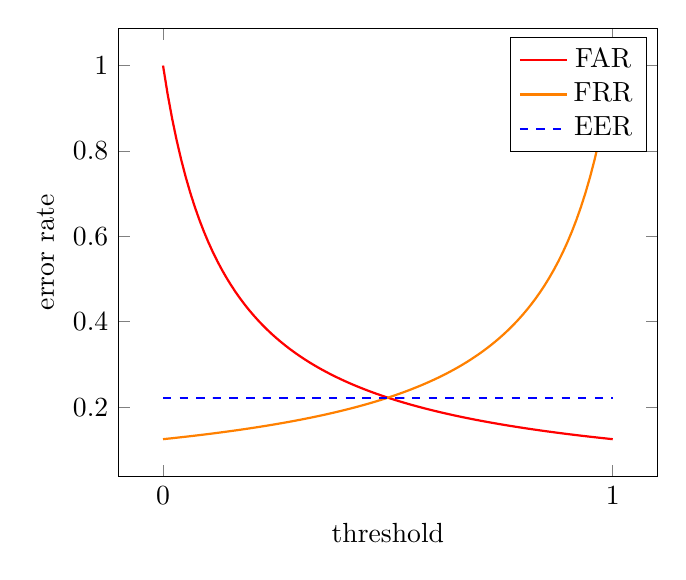
\begin{tikzpicture}
        \begin{axis}[
                xlabel=threshold,
                ylabel=error rate,
                xtick={1,8},
                xticklabels={0,1}
            ]
            \addplot[
                domain=1:8,
                samples=100,
                thick,
                color=red]{1/x};
            \addlegendentry{FAR};
    
            \addplot[
                domain=1:8,
                samples=100,
                thick,
                color=orange]{1/(9-x)};
            \addlegendentry{FRR};
    
            \addplot[
                domain=1:8,
                samples=100,
                dashed,
                thick,
                color=blue]{2/9};
            \addlegendentry{EER};
        \end{axis}
    \end{tikzpicture}
    \caption{\textit{False Acceptance Rate} and \textit{False Rejection Rate}
    for biometric authentication}
    \label{fig:eer}
\end{figure}

\section{Password Security}
Passwords which are short or badly chosen can easily be cracked. Brute-force or
dictionary attacks guess the password eighter randomly of from a list of known
(pass-)words. Brute-force attacks are easily feasible for passwords up to
\textasciitilde 8 characters in length, useful rules on possible guesses and
dictionary attacks can lead to success for even longer passwords. An advantage
for the attacker is when the attack can be executed \textit{offline}, such as by
stealing the file containing the password hashes. This removes the bottleneck of
the authentication mechanism of the target and allows for distributed attacks.

A common protection measure is to use a \emph{SALT}. A salt is a random value
that gets appended to the password before hashing, and then gets stored
alongside the password hash. While this does not protect a single password
against the mentioned attacks, it prevents reuse of a hash that has already been
calculated. Otherwise, it would be possible to just compare the hashes to known
hashes of popular passwords.

Another consideration is access to the password hashes. While the actual
cryptographic security is only influenced by the hash function, preventing
offline attacks by properly protecting the hashes forces the attacker to execute
much slower online attacks. Those online attacks can be slowed even further by
limiting the number of invalid authentication attempts or introducing an
increasing delay after failed authentication attempts (\textit{back off}), and
by using ``slow'' hash functions. The previously popular measure of password
aging (requiring passwords to be changed after a certain amount of time) is
discouraged, since it promotes the use of weak but easy to remember passwords.

Other attacks focus on the specific implementation of the authentication
mechanism and exploit vulnerabilities that allow login even without actually
obtaining the correct password, or allow changing or resetting passwords even
with insufficient privileges.

\subsection{Time Memory Trade-off}
In attacks on passwords a trade-off between time and memory has to be made, the
two extremes being the brute-force attack and the fully pre-calculated
dictionary/codebook attack.


\section{Network Authentication}

\chapter{Access Control}
Access control combines authentication and authorization.
\Cref{chapter:authentication} showed how the identity of a subject can be
confirmed, the question is now whether the subject is \emph{authorized} to
access a specific resource. This decision is generally performed by a
\emph{reference monitor}, on the basis of some \emph{access policy}, which may
be set by an administrator or the owner of the object.To differentiate the terms
\textit{subject} and \textit{object}:

A \emph{subject} is the \textit{acting entity}, which intends to carry out an
operation requiring access. Examples include persons, processes or network
nodes. A subject can also be the object of an access operation at another time.

An \emph{object} is the unit that is \textit{being accessed}. Examples include
files and directories, database records, computers, processes, mailboxes or
applications.

The \emph{access operation} is the type of operation of a subject in relation to
an object. Different sets of access operations can be defined. A file system
might for example define \textit{read} and \textit{write} operations (or
\textit{observe} and \textit{alter}). There might be additional operation like
\textit{execute} or \textit{append}, which can be handled independently.

\section{Access Control Matrix}
The access policy can be described using an \textit{access control matrix}. The
matrix contains the set of every allowed operation for every possible pair of
subject and object. This however immediately presents a problem, as this
approach scales badly. For $N$ subjects (users) and $M$ objects (files), a $N
\times M$ matrix would have to be stored.

Two implementations of the access control matrix may be more appropriate
depending on the application:

\subsection{Access Control List}
In an Access Control List (\textit{ACL}), a list of subject-operation pairs is
stored with each object. A file might for example contain a list of all users
that have access to that file, and which exact operations they are allowed to
execute on the file. If a user is not allowed to interact with the file in any
way, the entry may be omitted.

\subsection{Capabilities}
In direct contrast to the ACL, in a capabilities based system the subjects
contain a list of objects and the corresponding operations which the subject is
authorized to execute on the object. In the file system example, each user would
contain a list of files which the user is allowed to access.

\section{Models for Access Control}
More detailed access control models are in use:
\begin{itemize}
    \item[DAC] \emph{Discretionary Access Control} is the approach as explained
          above. Access control decisions are based on a subject and object.
          Subjects define the access rights of an object (file owner for
          example).
    \item[MAC] \emph{Mandatory Access Control} is oriented towards clearance
          levels, as one might expect in a government or military setting. The
          access rights are usually defined system-wide, and are not changed by
          a subject. More information on this in \cref{sec:belllapadula}.
    \item[RBAC] In \emph{Role Based Access Control} access to objects is not
          defined per subject, but per \textit{role}. Roles are given to
          subjects, and may change.
    \item[ABAC] \emph{Attribute Based Access Control} is even more abstract,
          where both subjects and objects have attributes, and access control
          decisions are made by flexible comparison of attributes.
\end{itemize}

Real world systems often implement aspects of multiple of those models, and no
model is the best or definitive answer to access control.

\section{Example: Linux}
\todo[inline]{Linux access control, ACLs}

\section{Multilevel Security, Bell-Lapadula-Model}
\label{sec:belllapadula}
In multilevel security, both objects and subjects are classified. Classes may
for example be \textit{Unclassified}, \textit{Confidential}, \textit{Secret} and
\textit{Top Secret}. Access is only granted if the subject has at least the same
classification as the object. Access is denied if the subject has a lower
classification than the object. The \emph{Bell-Lapadula-Model} is an
implementation of this access control model:

To define this model, consider a set of subjects $S$, a set of objects $O$ and
the set of operations $A = \{\text{execute}, \text{read}, \text{append},
\text{write}\}$. For two security levels $a, b \in SL$, there always exists a
greatest lower bound $l \in SL: (l \leq a, l \leq b \text{ and } l
\text{minimal})$ and a least upper bound $h$.

The system is in a state at all times. A state is a triple $(b, M, f)$ with
\begin{itemize}
    \item $b \subseteq S \times O \times A$ the set of current accesses
    \item $M = (M_{so})_{s\in S, o\in O}$ the current access matrix
    \item $f = (f_s, f_c, f_o)$ with
          \begin{itemize}
              \item $f_s: S \mapsto SL$ the maximum clearance of each subject
              \item $f_c: S \mapsto SL$ the current clearance of each subject
                    (this requires $f_c(s) \leq f_s(s)$ for each subject $s$)
              \item $f_o: O \mapsto SL$ the security classification of each
                    object
          \end{itemize}
\end{itemize}

The current clearance $f_c$ is chosen by each subject, within the limit set by
the maximum clearance $f_s$.

A state is secure, if the following properties are met:
\begin{itemize}
    \item \emph{Simple Security Property}: For all $(s, o, a) \in b$ with
          $a=\text{read}$ or $a=\text{write}$: $f_o(o) \leq f_s(s)$ (Each
          subject which is currently reading or writing has the necessary
          maximum clearance)
    \item \emph{*-Property}:
          \begin{itemize}
              \item For all $(s,o,a)\in b$ with $a=\text{append}$: $f_c(s) \leq
                        f_o(o)$ \\ (No append operation is executed with higher
                        clearance than the object)
              \item For all $(s,o,a)\in b$ with $a=\text{write}$: $f_c(s) =
                        f_o(o)$ \\ (Each write operation is executed with
                        minimal clearance)
              \item For all $(s,o,a)\in b$ with $a=\text{read}$: $f_c(s) \geq
                        f_o(o)$ \\ (Each read operation is executed with a
                        sufficient current clearance)
          \end{itemize}
          This property enforces the correct selection of the current clearance
          $f_c$. Appending happens ``upwards'', writing on the same level, and
          reading ``downwards''.
    \item \emph{Discretionary Security Property}: For all $(s,o,a) \in b$: $A
              \in M_{s,o}$
\end{itemize}

\section{POSIX Capabilities}
POSIX capabilities are an implementation of a capability based access control
scheme. An example would be the right to open raw sockets on linux, which is
usually reserved to the root user. This is however necessary for the
\texttt{ping} utility, which should be accessible to every user, even without
setting the \texttt{setuid} bit on the binary. The POSIX capability system now
allows giving the specific right to open raw sockets to the specific binary.
This also adheres to the principle of least privilege a lot better than always
executing \texttt{ping} with full root rights. Capabilities are also not
reserved to files, but can be given to individual processes as well.

\chapter{Malware}
\section{Buffer Overflow Attacks}
Buffer overflows are one of the main security vulnerabilities found today.
Modern mitigations make them not as trivial in practice as in theory. The most
common form is a \emph{stack overflow}. The goal is to overwrite the return
address of the current stack frame, usually by exploiting unchecked array-access
which allows writing to the address where the return address is located. The
attacker could instruct the program to return to a different part of the
program, for example skipping authentication checks. If write access to an
executable page is also present, the attacker could also first inject code and
then jump to that code, executing arbitrary instructions. If the place of the
injected shellcode is not known exactly, one technique is to insert \texttt{NOP}
instructions before the actual exploit (\textit{NOP sled}).

Mitigations include canaries, which are values placed between the variables and
return address on the stack to indicate buffer overflows. Injection of shellcode
is usually protected against by not allowing memory pages with both write and
execute permissions. Type-safe languages also offer features making access to
memory outside of variables impossible. Address space layout randomization makes
guessing memory locations more difficult.


\section{Introduction to Malware}
Malware is a generic term for software, which is designed to perform a function
undesirable or harmful to the user. Categorization of malware is possible by the
approach of spreading:
\begin{itemize}
    \item A \emph{virus} is a program which spreads by abusing other (harmless)
          programs
    \item A \emph{worm} spreads autonomously over a network
    \item A \emph{trojan} disguises itself as a harmless program
\end{itemize}

Especially malware that spreads over the network can be further categorized, the
main distinction being the amount of interaction a user has to perform in order
to be infected, which can lead from downloading and opening an attachment to
only visiting a website or even zero-interaction vulnerabilities.

Initial infection may also happen completely offline, for example via the ``lost
USB stick'' tactic in a more targeted attack.

The malicious payload can assume many forms and achieve a multitude of goals.
Some examples of payload functionality include:
\begin{itemize}
    \item Deleting data
    \item Spying, exfiltrating data
    \item Enabling remote access
    \item Denial Of Service (\textit{DOS})
    \item Physical damage
    \item Encryption of data (and demanding ransom)
    \item Abusing resources (crypto mining)
\end{itemize}

More often than not, those are motivated by financial gains, which is apparent
with the recent waves of large scale ransomware attacks.

Malware may also be categorized into mass infection and targeted attacks
(Advanced Persistent Threat \textit{APT}). While the former is focused entirely
on maximizing the number of infected hosts, the latter is focused on a specific
target.


\section{Botnets and Targeted Attacks}

Botnets are established with no particular payload. The initial infection
happens with a \textit{dropper}, which connects to a command and control server.
The actual payload is then downloaded from this server, which allows the botnet
to be rented out to perform a number of different attacks that all benefit from
a large amount of infected machines.

\chapter{OS Security}
\textit{Operating system-} and \emph{host-security} has the goals of protecting
stored data, running processes and the operating system itself. This
necessitates some form of authentication, to distinguish between users on a
multi-user system, as well as an access control system which assigns permissions
to users. A useful concept applied here is isolation, which is applied to users
and processes. Raw hardware access is usually restricted, and only allowed to
privileged code within the operating system. Protection against external access
may also be part of host security.

\section{Concepts and Reference Monitors}
A \emph{reference monitor} is an abstract machine which mediates all accesses to
objects by subjects (see \cref{chapter:access_control}). Reference monitors can
be implement on any level of the system. Reference monitors in the systems
hardware include the MMU and privileged execution modes. Kernel level reference
monitors are for example implemented in the file system or capability system.
Applications can also contain reference monitors, which may be the case in web
server applications, or run completely inside another program which implements a
reference monitor such as the Java virtual machine or a database engine.

The \emph{security kernel} is the hardware, firmware and software of a trusted
computing base which implements the reference monitor. It must mediate all
accesses, be protected from modification and be verifiable as correct.

The \emph{trusted computing base (TCB)} is the totality of protection mechanisms
within a computer system. This includes hardware, firmware and software which is
responsible for enforcing a security policy. The enforcement of the security
policy must only depend on the TCB, the rest of the operating system need not to
be trusted.

\section{Virtualization and Mandatory Access Control}
\subsection{Virtualization}
There exist many reasons to use virtualization, but the goal of virtualization
from a security perspective is full isolation of systems and applications. The
possibility to roll back an entire system to a known-good state in case of
compromise also presents an advantage.

Levels of virtualization are distinguished based on the role and position of the
\emph{virtual machine monitor VMM}. In \emph{native virtualization}, the VMM
directly interfaces with the hardware. In \emph{user mode virtualization}, the
VMM only interfaces with the host OS, and not directly with the hardware. A
hybrid approach is \emph{dual-mode virtualization}, where a host OS exists, but
some form of direct access to the hardware by the VMM is possible.

The interaction of the VMM with the \emph{guest OS} provides another way of
categorization: In \emph{full virtualization}, the guest OS runs unmodified, as
on real hardware. This is usually assisted by various hardware extensions such
as \textit{AMD-V} and \textit{Intel VT-x}, special support by the MMU and
passthrough of system busses such as PCI.

\emph{Paravirtualization} refers to a mode of virtualization in which the guest
OS is aware of the virtualization and has some adaptations to the host OS.
Hardware drivers for example can be replaced with components that directly
interface with the VMM.

\subsection{Isolation}
Isolation is the main benefit of virtualization from a security perspective.
Errors in applications can be contained effectively, programs with different
security requirements can be separated, and malware analysis is possible without
effecting the host system. The host system can employ detailed monitoring, and
perform effective intrusion detection from the outside. The isolation of common
dependencies between applications prevents the compromise of multiple
applications by compromise of the common dependency.

As an example, a payment processor may be located in a dedicated VM with a
secure operating system. The non-critical application such as a frontend which
exposes a large attack surface runs in a separate VM and interfaces with the
payment application only through a closely monitored interface.

\subsection{Security Enhanced Linux}

\section{Use-Case: iOS Security}

\chapter{Embedded and Hardware Security}

Security in embedded systems is of special concern. Embedded systems are often
harder to patch, and often have direct real-world impact, sometimes in a safety
critical way. Non-mainstream operating systems are in use, and the CPU might not
offer all desired security features (see below). This results in a large attack
surface on a system that is not as well understood security-wise as desktop- or
server applications.

In the following, security will be considered from a lower level than before,
down to the hardware. Many of the security measures considered before can be
circumvented if lower-level access is present. Access control on a file system
for example is worthless if the attacker can connect the disk to another system
and dump all the contents. Software security is difficult if it relies on
libraries that can be exchanged by an attacker.

Placing security mechanisms at the lowest possible layer circumvents those
attacks.

\section{Introduction and x86 Privilege Levels}
At any point while an x86 processor is executing instructions, it is in some
\emph{privilege level} or \emph{protection ring}, usually indicated by a number
where higher numbers represent less privileged execution. Switching to a lower
privilege level must be protected, while switching to a higher level (less
privileges) is usually easy. One important feature made possible by this is
protection of memory segments. Each memory segment contains a Descriptor
Privilege Level \textit{DPL}, and each process is assigned a privilege level. If
the Current Privilege Level \textit{CPL} > \textit{DPL}, the CPU generates a
protection fault and prevents access to memory accessible only to lower
privilege levels. This for example prohibits applications from modifying
operating system data structures.

Upgrading of the privilege level (setting it to a lower value) may happen for
example when a syscall is initiated and execution is passed to the operating
system. This provides a well defined ``gate'' to those privilege levels.

In order to prevent an application to misuse the privilege level of the syscall,
by for example instructing it to copy data into the process that the application
would otherwise not have access to, an additional \textit{Requested Privilege
Level} may be introduced (\emph{confused deputy problem}).


\section{Isolation and HW-based Attacks}
\section{HW-based Security Mechanisms}
\chapter{Software Security}
\todo[inline]{Chapter 8: Software Security}
\chapter{Network Security}
\todo[inline]{Chapter 9: Network Security}
\chapter{Web Security}
All components of a web application, the browser, the web server and the
underlying infrastructure are all subject to various attacks:

The \emph{connection} is vulnerable to misuse of TCP/IP mechanisms, such as
\textit{SYN flooding}. Eavesdropping and man-in-the-middle attacks are of
concern to any network connection, and as such also for web applications.

\emph{Web servers} or \emph{web applications} are often the target of an attack.
Various techniques such as XSS, injections and authentication bypasses are
explained later in this chapter.

Attacks against the \emph{browser} exploit flaws in the renderer, engine,
through scripting or plugins like java and flash.

\section{Transport Layer Security}
TLS presents a solution to secure TCP/IP connections. Its goals are to provide
authentication, protection, and confidentiality: Servers are authenticated using
X.509 certificates, clients can optionally authenticate the same way. The
transferred data is encrypted. TLS is implemented on top of TCP/IP and provides
an API very similar to normal TCP sockets.

\subsection{Handshake Protocol}
The TLS handshake protocol establishes a TLS session, including authentication,
negotiation of cryptographic primitives and negotiation of a symmetric session
key. One TLS session allows for multiple parallel TLS connections.

\begin{figure}
    \centering
    \begin{tikzpicture}
        \begin{umlseqdiag}
            \umlactor[class=Client]{c}
            \umlobject[class=Server]{s}
            \begin{umlfragment}[type=1, inner xsep=2, name=1]
                \begin{umlcall}[op={client hello}, dt=7]{c}{s}
                \end{umlcall}
                \begin{umlcall}[op={server hello}]{s}{c}
                \end{umlcall}
            \end{umlfragment}
            \umlnote[x=7, y=-2]{1}{Negotiation of security parameters (``ciphersuite'')}


            \begin{umlfragment}[type=2, inner xsep=2, name=2]
                \begin{umlcall}[op=certificate,dt=7]{s}{c}
                \end{umlcall}
                \begin{umlcall}[type=return, op={server key exchange}]{s}{c}
                \end{umlcall}
                \begin{umlcall}[type=return, op={certificate request}]{s}{c}
                \end{umlcall}
                \begin{umlcall}[op={server done}]{s}{c}
                \end{umlcall}
            \end{umlfragment}
            \umlnote[x=7, y=-4]{2}{Server authentication towards client}
            \umlnote[x=7, y=-6]{2}{Optional: key exchange and request for client certificate}

            \begin{umlfragment}[type=3, inner xsep=2, name=3]
                \begin{umlcall}[type=return, op={certificate},dt=7]{c}{s}
                \end{umlcall}
                \begin{umlcall}[op={client key exchange}]{c}{s}
                \end{umlcall}
                \begin{umlcall}[type=return, op={certificate verify}]{c}{s}
                \end{umlcall}
            \end{umlfragment}
            \umlnote[x=7, y=-8]{3}{Client key exchange}
            \umlnote[x=7, y=-10]{3}{Optional: certificate-based client authentication}

            \begin{umlfragment}[type=4, inner xsep=2, name=4]
                \begin{umlcall}[op={change cipher spec},dt=7]{c}{s}
                \end{umlcall}
                \begin{umlcall}[op={finished}]{c}{s}
                \end{umlcall}
                \begin{umlcall}[op={change cipher spec}]{s}{c}
                \end{umlcall}
                \begin{umlcall}[op={finished}]{s}{c}
                \end{umlcall}
            \end{umlfragment}
            \umlnote[x=7, y=-12]{4}{Switch to encryption}
        \end{umlseqdiag}
    \end{tikzpicture}
    \caption{TLS Handshake Protocol}
    \label{fig:tls_handshake}
\end{figure}

\begin{figure}
    \centering
    \begin{tikzpicture}
        \begin{umlseqdiag}
            \umlactor[class=Client]{c}
            \umlobject[class=Server]{s}
                \begin{umlcall}[op={client hello}, dt=7]{c}{s}
                    \begin{umlcall}[op={client random},dt=5]{c}{s}
                    \end{umlcall}
                    \begin{umlcall}[op={suggested cipher suites}]{c}{s}
                    \end{umlcall}
                    \begin{umlcall}[op={suggested compression}]{c}{s}
                    \end{umlcall}
                    \begin{umlcall}[op={session ID: 0x00}]{c}{s}
                    \end{umlcall}
                \end{umlcall}
                \begin{umlcall}[op={server hello}]{s}{c}
                    \begin{umlcall}[op={server random},dt=5]{s}{c}
                    \end{umlcall}
                    \begin{umlcall}[op={use cipher suites}]{s}{c}
                    \end{umlcall}
                    \begin{umlcall}[op={session ID}]{s}{c}
                    \end{umlcall}
                \end{umlcall}
        \end{umlseqdiag}
    \end{tikzpicture}
    \caption{TLS Handshake Protocol: Hello messages (phase 1)}
    \label{fig:tls_hello}
\end{figure}

\Cref{fig:tls_handshake} shows an overview of the TLS handshake: In \emph{phase
1}, the client offers a list of supported cipher suites to the server. The
server selects a cipher suite, and establishes a session ID. Random values for
later key creation are also exchanged. \Cref{fig:tls_hello} shows phase 1 in
detail.

In \emph{phase 2}, the server sends its certificate, and optionally requests a
client certificate for authentication of the client.

In \emph{phase 3}, the client sends its certificate, if requested. The client
has verified the server using the certificate, and can now use the severs public
key for establishing a symmetric session key. The client generates a
\texttt{PreMasterSecret}, from which client and server can derive the symmetric
key using the random values exchanged in phase 1. The \texttt{PreMasterSecret}
is RSA-encrypted using the servers public key and then sent to the server.

In \emph{phase 4}, the symmetric session key is established. The integrity of
the handshake is verified by exchanging hashes over the derived key and the
previous messages. All following communication happens encrypted.

\subsection{Record Protocol}
Once the handshake is complete, the handshake protocol takes over and handles
transfer of data. The record protocol is completely separate to the handshake
protocol, making it theoretically possible to execute the handshake completely
offline. The record protocol handles, in order: Fragmentation, Compression,
Message Authentication Code, Encryption. Receiving works the same way in the
opposite order. MAC and encryption use separate keys for both directions.

\section{Injection Attacks}
In injection attacks, some specially crafted input to the web application leads
to unwanted effects.

\subsection{Cross Site Scripting}
Many web applications accept some kind of textual input, which then gets shown
to a different user on the website, such as a forum- or social media post. If no
special care is taken, this means that anyone can place arbitrary HTML,
including scripts, on the website in the targets browser. This is referred to as
\textit{Cross Site Scripting} or \emph{XSS}. A typical goal of such an attack is
to steal cookies, which might allow the attacker to take over the login session
of the target. Exfiltration of the cookie might happen via the query parameters
of an image that gets loaded from the attackers server via the injected script.
Protection against those kinds of attack include validating the input, and
removing possibly dangerous characters, or making sure that user generated
content is only interpreted as text by the browser, and not executed. Other
measures include instructing the targets browser to not make any request to
external servers, which hinders exfiltration.

\subsection{SQL Injection}
User inputs such as login credentials are often used as parts of SQL queries. If
the input contains valid SQL syntax, and is just appended to a query, it might
change the query in a way such that it always returns a certain value to bypass
authentication, or execute arbitrary statements with the privilege of the web
server application. Even escaping the input data might not solve the issue, as
second order injections might circumvent that. Again, it is important to ensure
input data is only handled as text and no situation exists where it is
potentially executed as code.

\chapter{Data Protection and Privacy}
\section{Privacy Motivation}
\todo[inline]{privacy motivation}

\section{Privacy by Design and PETs}
\subsection{Anonymous Communication: TOR}
TOR implements a form of onion routing and a mix-network: A message for a server
is encrypted with its public key. It is however not directly sent to this
server, but through another server, which requires an additional layer of
encryption for the intermediate server. (In practice, this asymmetric encryption
may be replaced by a key exchange and symmetric encryption for the actual data,
for performance reasons). This is repeated such that there are three
intermediate \textit{onion routers} between the source and destination. This
way, none of the routers sees both the source and destination: The first router
knows about the source, the last router knows about the destination, the middle
router does not know the source or destination.

Attacks are possible by correlation of packets inside the network, incorrect
usage of DNS or identification by the message payload.

\subsection{Blind Signatures}
A blind signature is needed when a document shall be signed without revealing it
to the signing party. This works by first ``blinding'' the message, signing the
blinded message, then unblinding the signed, blinded message. This results in a
signed form of the original message.

These kind of blind signatures are useful for electronic cash, which should
provide anonymity, verifiable authenticity and protection against double
spending. An analogy works as following: The user who wants to spend money puts
an empty piece of paper with carbon paper in a sealed envelope. The bank signs
that envelope on the outside, which makes the envelope with the paper inside
worth 1\$. While signing the envelope, the signature was printed on the paper
inside the envelope. This signed paper is now used as payment. The bank has
however not seen the actual paper inside the envelope. Double spending is
prevented by containing a serial number on the paper, which the merchant
verifies with the bank before accepting payment.

\subsection{Group Signatures}
A group of users has a shared public key, but each user has an individual
private key. A message should now be signed with a private key, and verification
should be possible via the group public key. Group anonymity is provided since
it is only confirmed during validation that a member of the group produced the
signature, but not which exact member.

A problem is that the group manager, who issues keys to the members, can spoof
any participants identity and acts as a kind of trusted third party. The group
manager might also be able to identify the individual member from a signature.

\subsection{Attribute-Based Credentials}
Using \emph{Attribute Authentication}, the user can provide proof of an
attribute without revealing their own identity. Multiple authentications should
not be linkable. Examples could include public transport tickets, where the
owner should only be required to prove authorization to travel on the current
route, without revealing identity or entire travel plans. ABCs can also
implement pseudonymous or not-at-all-anonymous authentication.

In an ABC scenario, the ABC authority first authorizes an issuer, and issues a
device (smartcard) to the user. The issuer can then issue credentials containing
attributes stored on the card. The card can then generate a selective proof
revealing some attribute to a relying party.

\end{document}